%%%%%%%%%%%%%%%%%%%%%%%%%%%%%%%%%%%%%%%%%%%%%%%%%%%%%%%%%%%%%%%%%%%%%%%%%%%%%%%
%
%    NEPI, a framework to manage network experiments
%    Copyright (C) 2013 INRIA
%
%    This program is free software: you can redistribute it and/or modify
%    it under the terms of the GNU General Public License as published by
%    the Free Software Foundation, either version 3 of the License, or
%    (at your option) any later version.
%
%    This program is distributed in the hope that it will be useful,
%    but WITHOUT ANY WARRANTY; without even the implied warranty of
%    MERCHANTABILITY or FITNESS FOR A PARTICULAR PURPOSE.  See the
%    GNU General Public License for more details.
%
%    You should have received a copy of the GNU General Public License
%    along with this program.  If not, see <http://www.gnu.org/licenses/>.
%
% Author: Alina Quereilhac <alina.quereilhac@inria.fr>
%
%%%%%%%%%%%%%%%%%%%%%%%%%%%%%%%%%%%%%%%%%%%%%%%%%%%%%%%%%%%%%%%%%%%%%%%%%%%%%%%

% Motivation
During the past decades, a wide variety of platforms to conduct network
experiments, including simulators, emulators and live testbeds,
have been made available to the research community.
Some of these platforms are tailored for very specific use cases (e.g.
PlanetLab for very realistic Internet application level scenarios), 
while others support more generic ones (e.g. ns-3 for controllable 
and repeatable experimentation). Nevertheless, no single platform is 
able to satisfy all possible scenarios, and so researchers often rely 
on different platforms to evaluate their ideas.

Given the huge diversity of available platforms, it is to be expected a
big disparity in the way to carry out an experiment between one platform and 
another. Indeed, different platforms provide their own mechanisms to 
access resources and different tools to conduct experiments. 
These tools vary widely, for instance, to run a ns-3 simulation it is 
necessary to write a C++ program, while to conduct an experiment using
PlanetLab nodes, one must first provision resources through a special web
service, and then connect to the nodes using SSH to launch any applications
involved in the experiment.

Mastering such diversity of tools can be a daunting task, 
but the complexity of conducting network experiments is not only limited 
to having to master different tools and services.
Designing and implementing the programs and scripts to run an experiment
can be a time consuming and difficult task, specially if distributed
resources need to be synchronised to perform the right action at the
right time. Detecting and handling possible errors during experiment
execution also posses a challenge, even more when dealing with large size
experiments. Additionally, difficulties related to instrumenting the 
experiment and gathering the results must also be considered.

% Challenge
In this context, the challenges that NEPI addresses are manifold. 
Firstly, to simplify the complexity of running network experiments. 
Secondly, to simplify the use of different experimentation platforms, 
allowing to easily switch from one to another. 
Thirdly, to simplify the
use of resources from different platforms at the same time in 
a single experiment.

% How?
The approach proposed by NEPI consists on exposing a generic API
that researchers can use to \emph{program} experiments, and 
providing the libraries that can execute those experiments on 
target network experimentation platforms. The API abstracts the
researchers from the details required to actually run an experiment
on a given platform, while the libraries provide the code to 
automatically perform the steps necessary to deploy the experiment 
and manage resources.

The API is generic enough to allow describing potentially any 
type of experiment, while the architecture of the libraries was 
designed to be extensible to support arbitrary platforms.
A consequence of this is that any new platform can be supported in 
NEPI without changing the API, in a way that is transparent 
to the users.

% 
\section{Experiment Description}

NEPI represents experiments as graphs of interconnected resources.
A resource is an abstraction of any component that takes part of an 
experiment and that can be controlled by NEPI. 
It can be a software or hardware component, it could be a virtual 
machine, a switch, a remote application process, a sensor node, etc.

Resources in NEPI are described by a set of attributes, traces and 
connections. The attributes define the configuration of the resource,
the traces represent the results that can be collected for that resource
during the experiment and the connections represent how a resource relates
to other resources in the experiment.

\begin{figure}[h]
  \centering
  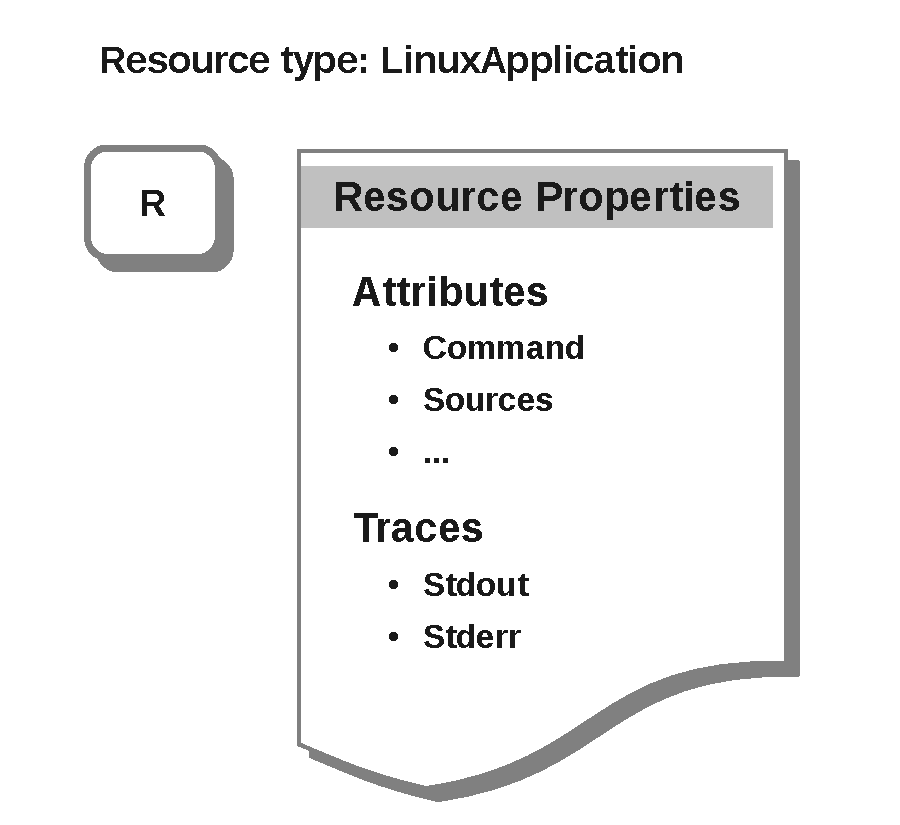
\includegraphics[width=0.5\textwidth]{intro_resource}
  \caption{Properties of a resource of type LinuxApplication}
  \label{fig:intro_resources}
\end{figure}

Examples of attributes are a linux hostname, an IP address to be 
assigned to a network interface, a command to run as a remote application.
Examples of traces are the standard output or standard error of a
running application, a tcpdump on a network interface, etc.

Resources are also associated to a type (e.g. a Linux host, 
a Tap device on PlanetLab, an application running on a Linux host, etc).
Different types of resources expose different attributes and traces
and can be connected to other specific types (e.g. A resource representing
a wireless channel can have an attribute SSID and be connected to a 
Linux interface but not directly to a Linux host resource)
Figure \ref{fig:intro_resources} exemplifies this concept.

There are two different types of connections between resources, the 
first one is used to define the \emph{topology graph} of the experiment.
This graph provides information about which resources will interact
with which other resources during the experiment
(e.g. application A should run in host B, and host B will be connected
to wireless channel D through a network interface C).
Figure \ref{fig:intro_topo_graph} shows a representation of the concept of
topology graph to describe the an experiment.

\begin{figure}[h]
  \centering
  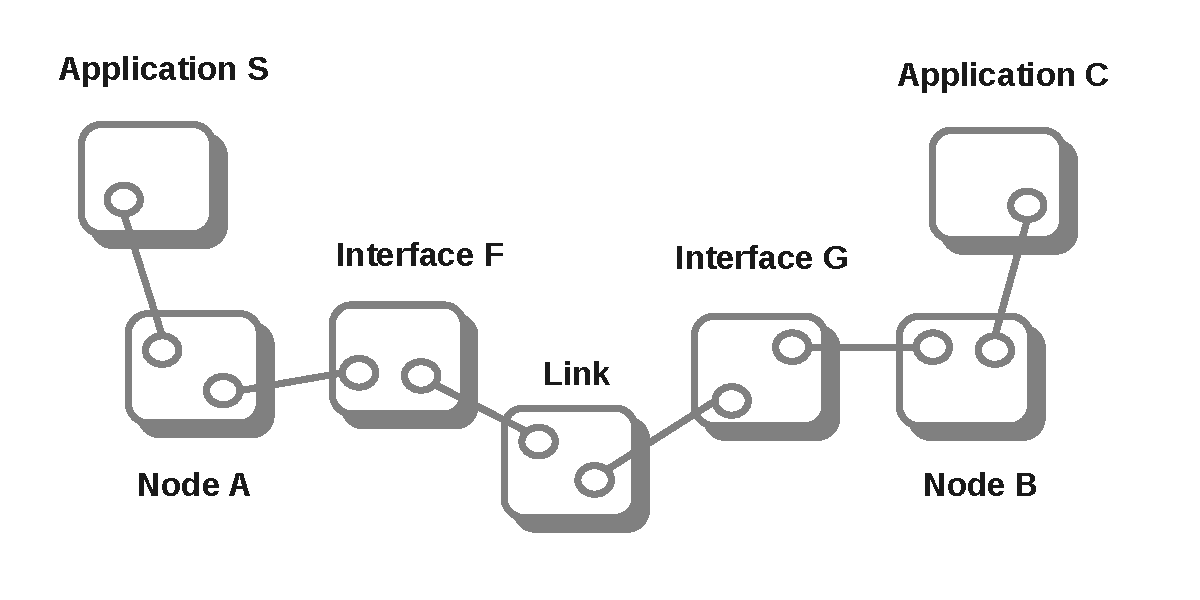
\includegraphics[width=0.8\textwidth]{intro_topo_graph}
  \caption{A topology graph representation of an abstract experiment}
  \label{fig:intro_topo_graph}
\end{figure}

The second type of connections (called conditions to differentiate them 
from the first type) specifies the \emph{dependencies graph}. 
This graph is optional and imposes constraints on the experiment 
workflow, that is the order in which different events occur during the 
experiment. For instance, as depicted in Figure \ref{fig:intro_dependencies_graph}
a condition on the experiment could specify that
a server application has to start before a client application does, or that
an network interface needs to be stopped (go down) at a certain time after
the beginning of the experiment. 

\begin{figure}[h]
  \centering
  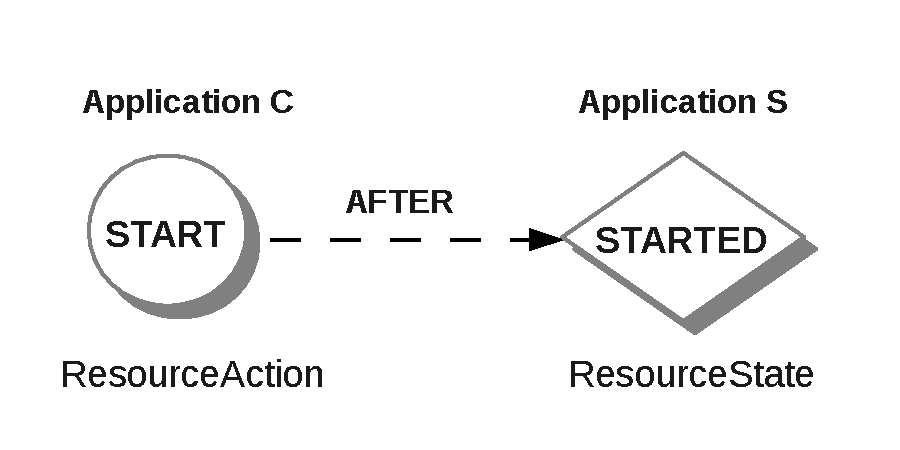
\includegraphics[width=0.8\textwidth]{intro_dependencies_graph}
  \caption{A dependencies graph representation involving two applications 
    resources in an experiment}
  \label{fig:intro_dependencies_graph}
\end{figure}

It is important to note, that the \emph{topology graph} also defines 
implicit and compulsory workflow constraints
(e.g. if an application is \emph{topologically} connected to a host,
the host will always need to be up and running before an application 
can run on it). 
The difference is that the \emph{dependency graph} adds complementary
constraints specified by the user, related to the behavior of the 
experiment.

This technique for modeling experiments is generic enough that can be used 
to describe experiments involving resources from any experimentation 
environment (i.e. testbed, simulator, emulator, etc). However, it
does not provide by itself any information about how to actually deploy
and run an experiment using concrete resources. 


\section{Experiment Life Cycle}

The Experiment Description by itself is not enough to conduct an experiment.
In order to run an experiment it is necessary to translate the description 
into concrete actions and to perform these actions on the specific resources
taking part of the experiment. NEPI does this for the user in an automated
manner.

\begin{figure}[h]
  \centering
  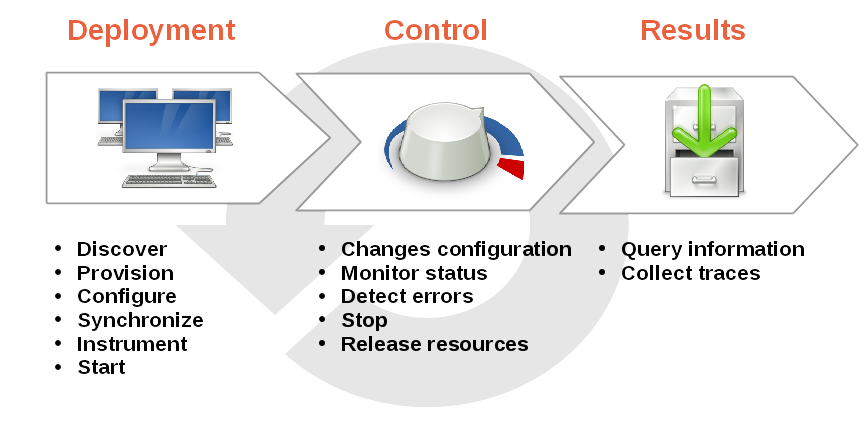
\includegraphics[width=0.8\textwidth]{intro_life_cycle}
  \caption{Common stages of a network experiment life cycle}
  \label{fig:intro_life_cycle}
\end{figure}

Given that different resources will require performing actions in 
different ways (e.g. deploying an application on 
a Linux machine is different than deploying a mobile wireless robot), 
NEPI abstracts the life cycle of resources into common stages associated
to generic actions, and allows to plug-in different implementation of 
these actions for different types of resources.
Figure \ref{fig:intro_life_cycle} shows the three
main stages of the network experiment life cycle, \emph{Deployment}, 
\emph{Control} and \emph{Result (collection)}, and the actions that are 
involved in each of them. 

\begin{figure}[h]
  \centering
  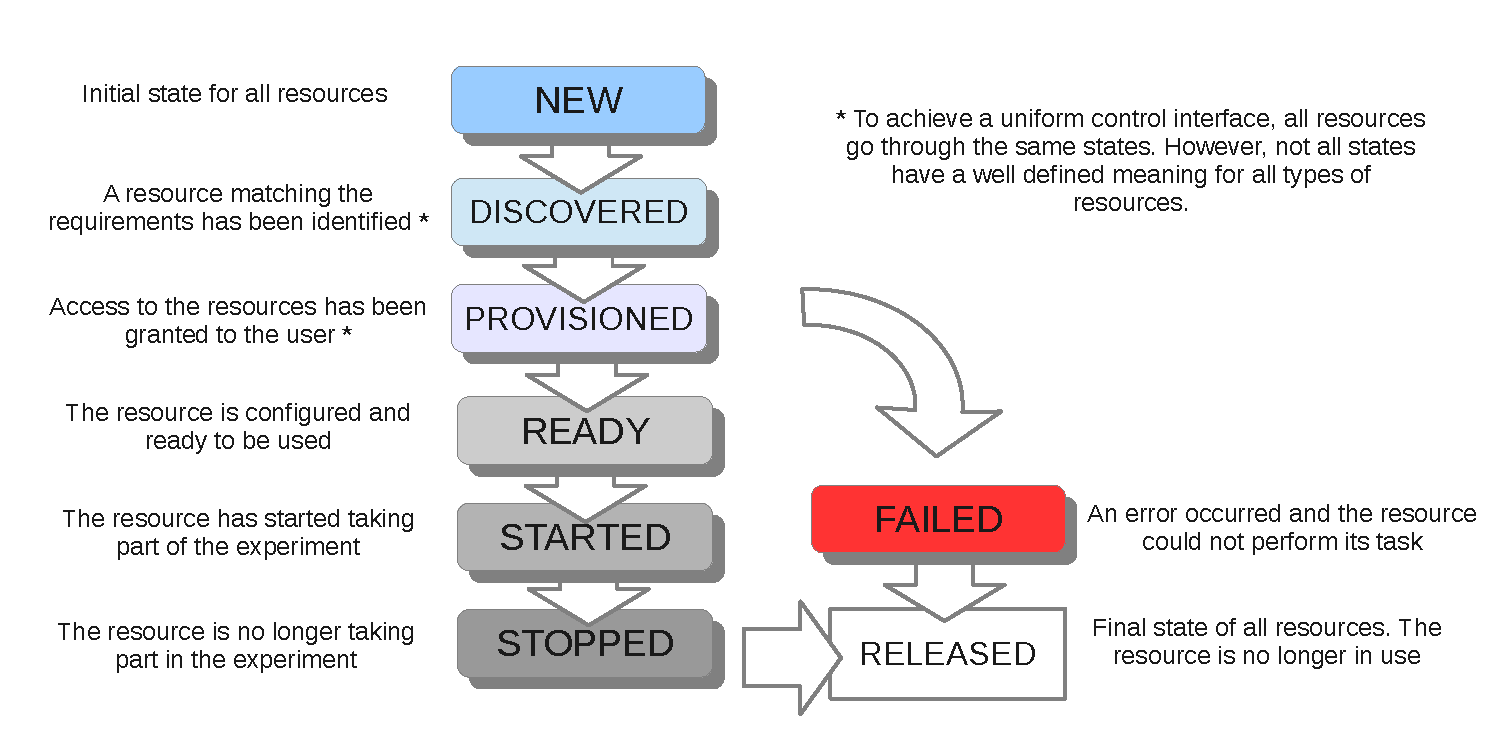
\includegraphics[width=\textwidth]{intro_state_transitions}
  \caption{Resources state transitions}
  \label{fig:intro_state_transitions}
\end{figure}

In order to be able to control different types of resources in 
a uniform way, NEPI assigns a generic state to each of these
actions and expects all resources to follow the same set of
state transitions during the experiment life. The states and
state transitions are depicted in Figure 
\ref{fig:intro_state_transitions}.

It is important to note that NEPI does not require these states
to be globally synchronized for all resources (e.g. resources
are not required to be all ready or started at the same time).
NEPI does not even require all resources to be declared and known 
at the beginning of the experiment, making it possible to use 
an \emph{interactive deployment} mode, where new resources can de 
declared and deployed on the fly, according to the experiment needs.
This interactive mode can be useful to run experiments with the 
purpose of exploring a new technology, or to use NEPI as an adaptive
experimentation tool, that could change an experiment according to
external conditions or measurements. 

\section{Resource Management: The EC \& The RMs}

The Experiment Controller (EC) is the entity that is responsible for 
translating the Experiment Description into a running experiment.
It holds the \emph{topology} and \emph{dependencies} graphs, and it 
exposes a generic experiment control API that the user can 
invoke to deploy experiments, control resources and collect results. 

\begin{figure}[h]
  \centering
  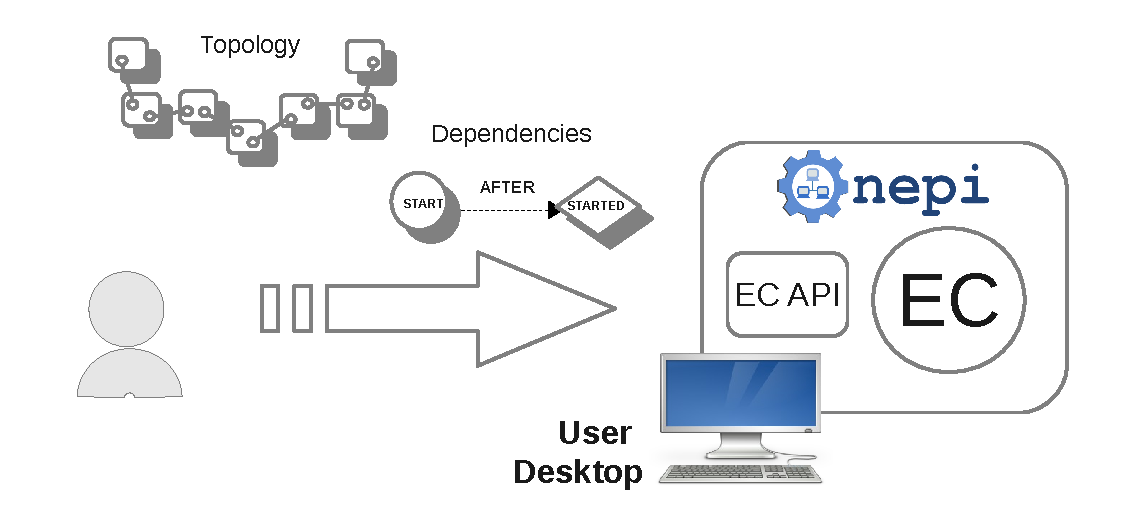
\includegraphics[width=\textwidth]{intro_ec}
  \caption{User interacting with the Experiment Controller}
  \label{fig:intro_ec}
\end{figure}

As shown in Figure \ref{fig:intro_ec}, the user declares the resources and
their dependencies directly with the EC. 
When the user requests the EC to deploy a certain resource or a
group of resources, the EC will take care of performing all the necessary 
actions without further user intervention, including the sequencing of 
actions to respect user defined and topology specific dependencies, 
through internal scheduling mechanisms. 

The EC is a generic entity responsible for the global orchestration of
the experiment. As such, it abstracts itself from the details of how to
control concrete resources and relies on other entities called Resource Managers 
(RM)s to perform resource specific actions. 

For each resource that the user registers in the \emph{topology graph}, the EC
will instantiate a RM of a corresponding type. A RM is a resource specific
controller and different types of resources require different type of
RMs, specifically adapted to manage them.

The EC communicates with the RMs through a well defined API that exposes
the necessary methods (actions) to achieve all the state transitions defined by the
common resource life-cycle. Each type of RM must provide a specific implementation
for each action and ensure that the correct state transition has been achieved
for the resource (e.g. upon invocation of the START action, the RM must take 
the necessary steps to start the resource and set itself to state STARTED).
This decoupling between the EC and the RMs makes it possible to extend the 
control capabilities of NEPI to arbitrary resources, as long as a RM can be 
implemented to support it.

As an example, a testbed \emph{X} could allow to control host resources using a 
certain API X, which could be accessed via HTTP, XMLRPC, or via any other protocol.
In order to allow NEPI to run experiments using this type of resource, it would
suffice to create a new RM of type host X, which extends the common RM API, and
implements the API X to manage the resources.

Figure \ref{fig:intro_resource_management} illustrates how the user, the EC, 
the RMs and the resources collaborate together to run an experiment.

\begin{figure}[h]
  \centering
  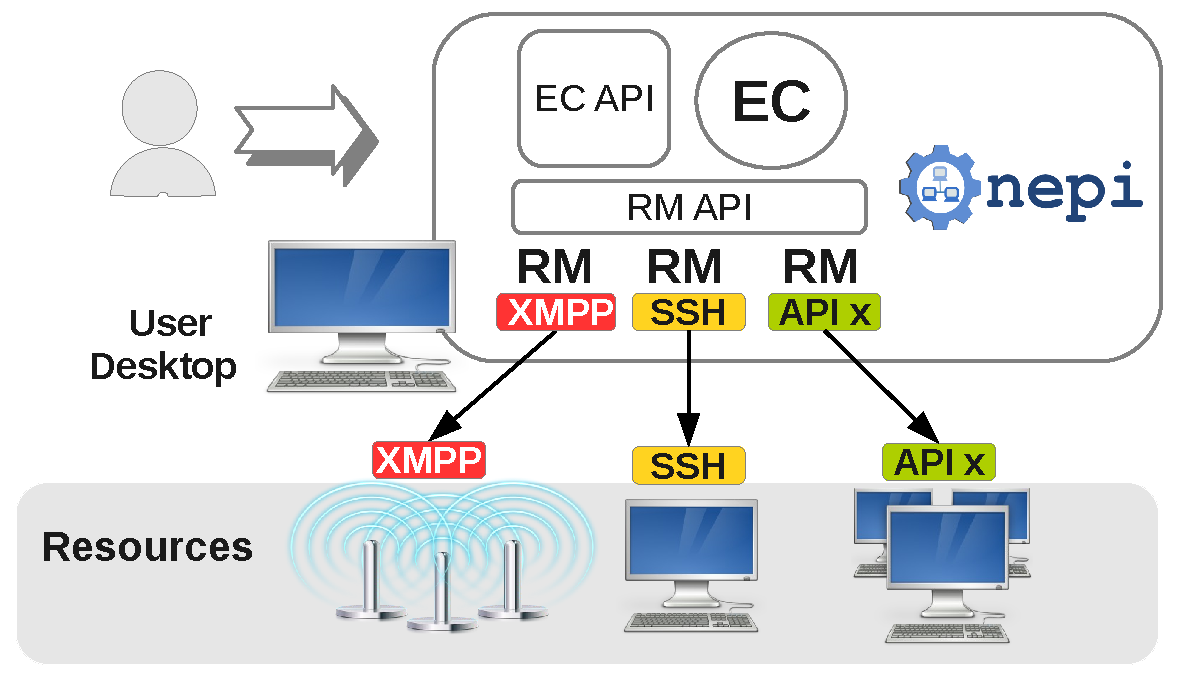
\includegraphics[width=\textwidth]{intro_resource_management}
  \caption{Resource management in NEPI}
  \label{fig:intro_resource_management}
\end{figure}
